\thesischapter{Background: Traditional Railway Control Systems:}
The birth of the railways occurred in the 1800s and from that point until the present day they have experienced continual growth, change and development. In the beginning the burden of safety was placed solely on human shoulders and has since been placed on mechanical systems before finally being transferred to electronics systems that are in place guaranteeing safety today. In the following we shall present a brief history of the railway followed by information on our industrial partner Invensys Rail.  Following this general introduction we shall look into specific equipment found on the modern railway and other information needed to understand the domain. Most importantly we shall describe the Westrace interlocking, a modern system charge with guaranteeing safety on the railway, which is produced by Invensys. In the final part of this chapter we shall look at some previous work in this field.


\begin{comment}
From their birth in the 1800s to the present day, the railway and its control
systems have seen many advances. Its control and safety has gone from being a
completely manual human based system, to a mechanical system and finally to the electronic
system we see today. We will now look at a brief history of the railway
followed by information on our industrial partner Invensys Rail. We then look
more closely at modern railways and the equipment which constitutes
them. We also study
Westrace interlocking which is produced by Invensys and the
ladder logic programs which run on it. Finally, we look at some previous work
in this field.
\end{comment}

\section{ A History of Railway Signalling and Control Systems}
Initially in the early days of the railway there was not fixed signals as we see today. Instead Policemen stationed at junctions and railway stations, were charged with signalling train drivers using a system of flags or oil lamps and changing the points of the railway. A major problem of the time, without telecommunications, was that there was no way of locating a train once it went out of sight. This meant that in practice the only safety precaution that could be taken was to delay the departure of trains using an egg timer which would hopefully space out their positions along the track. The level of safety resulting from this precaution was acceptable as train speeds were not relatively high at the time.


\begin{comment}
Prior to the days of fixed signals, Policemen would be stationed at
junctions and railway stations. They changed points manually and gave instructions to train drivers
by using a system of either flags or oil lamps depending on the
visibility. Since this was before the time of telecommunications and
electricity there was no way of telling where a train was once it left a
station and went out of sight. The only safety precaution that could be taken
was to use an egg timer to delay the departure of the next train in order to
give the previous train time to progress along the track. Train speeds were
not very high during this period so this was an acceptable way of ensuring safety.
\end{comment}


The most important type of signal found in the modern railway is the \textbf{fixed signal} which are static, positioned by the side of the track and visually present information to the train driver. The first fixed signals were wooden boards shaped in such a way to provide specific information attached to poles which rotate around a vertical axis. Typically these boards would form a signal instructing the train driver to stop, however if the board was rotated side-on to the driver then it becomes inactive and the driver would proceed if it is safe to do so.

\begin{comment}
Modern railway signally makes use of \textbf{fixed signals}. These are permanently positioned
by the side of the track and provide some visual information to the train driver.
The original fixed signal consisted of a shaped wooden board that could be
rotated on pole round a vertical axis. If the board was visible to the driver
then he would have to stop the train. On the other hand if the driver couldn't
see the board because it was side-on to him then he would be able to
proceed.
\end{comment}

The next major enhancement of these signals came in the form of the \textbf{Semaphore} fixed signal.  Instead of having 2 positions (visible/ not visible), the boards of a semaphore signal could be moved into one of several predetermined positions. The 
\begin{comment}
One of the major developments in railway signalling was the introduction of
the \textbf{Semaphore} fixed signal. These consisted of a board that could be
moved into several preset positions. Typically these would have  3 different visible
``aspects'' which they could be set to: One aspect to indicate the driver can
proceed, another that indicates the driver can proceed with caution and
finally an aspect which indicates that the driver should stop. 
\end{comment}



Around about the same time as the introduction of the semaphore signal, the system
for controlling the signals went under drastic change. The Policemen were
replaced with professional \textbf{Signallers} whose job was specifically to
manage the railways. A system of pulleys, wires and levers was also devised
to allow multiple signals and points to be controlled from a central
position. This central position became known as a \textbf{signal box} and was
manned by one or more signallers. This centralisation allowed for further
safety mechanisms to be installed. One in particular, namely the \textbf{interlocking},
is of interest to us. The interlocking physically locked levers if they were
unsafe to move.

The next leap in railway technology came from the invention of the electronic
\textbf{track circuit}. These would activate an indicator in the signal box if a
segment of track was occupied by a train. As more and more track circuits
became installed it was no longer necessary to have human intervention to
control certain signals. \textbf{Automatic signals} were introduced which
operated completely by track circuits without any intervention from human
signallers. Around this time \textbf{electric point machines} were introduced
removing a large amount of physical work performed by signallers allowing for
a greater area of control for each signaller.  Around this time
electromechanical \textbf{relays} began to replace purely mechanical relays
reducing the amount of space needed for a signal box.

In the 1920s \textbf{colour light signals} replaced mechanical semaphore signals these where much brighter than the oil
lamps fitted to semaphores and greatly increased the safety of night time
train travel. In the 1930s the mechanical levers were replaced with an electronic \textbf{control panel}
containing switches and buttons. This allowed for the introduction of
\textbf{route setting} where with the press of a button configurations of signals and points would be
associated with a particular route could become activated. Prior to this time
many levers would have had to have been pulled to set many different pieces of equipment.
During the 1980s the most important advance from our point of view took
place. The advent of electronic microprocessors enabled the replacement of the
relay and mechanical interlockings with an electronic \textbf{solid state interlocking}
system (SSI) \cite{AC08}. The main focus of this project will be to investigate the safety
of such solid state interlockings.

\section{Invensys Rail}

Invensys Rail \cite{Inven} and its previous incarnation Westinghouse Rail Systems Ltd have been
involved for over 140 years in producing equipment to increase safety in the
railway industry. Originally they produced air brakes for trains, these had a
failsafe state such that if the power was cut the brakes would automatically stop the train.
Later on in the company's development they provided support to British Rail
when the first solid state digital railway interlocking was installed in
Leamington Spa. Today they supply railway control equipment to companies based
around the globe, including companies based in Australia, Hong Kong,
Germany, Spain and the UK. This project is mainly concerned with one of the
solid state railway interlockings Invensys produces called the Westrace. The
Westrace railway interlocking continuously runs a ladder logic program which
prevents the railway control systems from entering a dangerous state. Ladder
logic will be explained in a later chapter.
David Kerr and Tony Rowbotham  produced a book that explains the
terminology and methodology used in the railway industry and by
Invensys (See \cite{KR01}).  

\section{An Overview of the Railway Domain} 
In this section we present the features of the railway domain that are in
the scope of this thesis. We hope to provide the reader with the background
information and terminology necessary to understand the parts of this thesis.


\subsection{The Railway Topology: Track and Points}
We will now present an overview of the physical railway from a topological
point of view. To do this we will present an example of a small track plan
of a junction.  If the reader is interested in learning more about the
topology of the railway a more detailed description can be found in \cite{KR01} 


\begin{figure}

\begin{center}

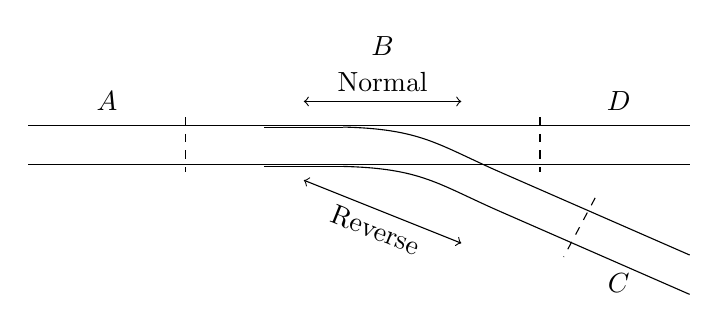
\begin{tikzpicture}

\node at (-4 , 1.3)  {$A$};

\node at (-0.5 , 2) {$B$};

\node at (2.5 , -1) {$C$};

\node at (2.5 , 1.3) {$D$};


\draw[<->] (-1.5, 1.3) to node [above, sloped] {Normal} (0.5 , 1.3) ;

\draw[<->] (-1.5 , 0.3) to  node [below, sloped] {Reverse} (0.5, -0.5);


\draw (-5, 1) -- (3.4,1);




\draw [dashed] (-3 , 1.1)  -- (-3, 0.4);

\draw [dashed] (1.5 , 1.1) -- (1.5 , 0.4);

\draw [dashed] (2.2 , 0.075) -- (1.8, -0.675) ;

\draw (-2, 0.975) -- (-1, 0.975);

\draw (-1, 0.975) .. controls (0, 0.95) and (0.2 , 0.75)  .. (1, 0.4);

\draw (1, 0.4) -- (3.4, -0.65);



\draw (-5, 0.5) -- (3.4, 0.5);

\draw( -2, 0.475) -- (-1, 0.475);

\draw (-1, 0.475) .. controls (0, 0.45) and (0.2 , 0.25)  .. (1, -0.1);

\draw (1, -0.1) -- (3.4, -1.15);





\end{tikzpicture}

\end{center}
\caption{A Typical Junction}

\label{fig:track}

\end{figure}


\subsubsection{Track Segments}
A section of track is typically broken down into track segments each
containing one or more track circuits to detect the presence of a
train. Typically track segments become larger on long straight stretches of
track without any interesting topological features such as junctions or
stations. Likewise track segments become smaller around junctions and stations
where control over train movement is of greater importance. 

\subsubsection{Points}
A point is a physical piece of equipment that is used to 
form a junction. Due to the nature of the rails and trains it is not possible to physically
to just join two segments of track. Instead a point is needed to act as
physical switch controlling the flow of trains through a junction. A point
has two positions which are referred to as \textbf{normal} and
\textbf{reverse}. This presents a safety hazard, for example see figure 2.1, if a train enters
the junction $b$ from $c$ when the junction is locked in the
position for normal then the train will be derailed. 



\subsection{Railway Signalling}
Signals are the main means used to communicate information regarding the state
of the track ahead of the train. Typically they are placed either on the track
side or over hanging the railway. Visual indications known as aspects are used
to convey information to the driver. A signal will have many such aspects
which can be displayed, each with a particular meaning. The main type of signal
considered in this project is the coloured light signal. Typically these have
between one - four aspects each conveying a different indication about the state of
the track ahead. Below is a description of the
aspects used for a three light signal.  


\begin{figure}[h!]
\begin{description}

\item[Green] - If this aspect is displayed it indicates that track ahead is
  clear for a sufficient distance and the train driver
  can proceed at full speed to the next signal.

\item[Yellow] - This aspect indicates the track immediately ahead in between
  this signal and the next is clear however the driver should proceed with
  caution as a train could be in the track after that.

\item[Red] - This aspect indicates that the track ahead is not clear, the
  driver should stop and wait at this signal.

\end{description}
\label{fig:3lightsignal}


\end{figure}

The one aspect signal is typically a fixed red indicating that is not possible
to proceed down the track at this current point in time. The two - four aspect
signals are used on tracks with different speeds to convey different stopping
distances.  The two aspect signal for instance would be used on a low speed
track segment where stopping distances are relatively short. Whereas the four
aspect signal would be used on a high speed line where stopping distances are
long and the driver needs information for a greater length of track. These
signalling schemes are fixed in the UK however they are not fixed from country
to country. On the continent, for example, they may use different conventions,
colours and number of lights on each signal.




\subsection{The Westrace Interlocking}

The railway interlocking is a key component in ensuring the safety of the
railway. Its job is to apply a set of rules to the requests and commands it receives from the
control system and check whether or not the future state of the railway is safe.
If the control signals it receives do not violate the safety of the railway
then these signals are committed to the physical infrastructure. For example if
the human controller requests for a route to be set the interlocking will
process this request and ensure that it does not conflict with other routes
before allowing the command to be passed to the physical railway.

\begin{figure}[h!]

\begin{center}
\begin{tikzpicture}[node distance = 2cm]

\tikzstyle{box2}=[box3,text width= 5cm,font=\small]
\tikzstyle{arrow}=[->,very thick,shorten >=7pt,shorten <=7pt]


\node (A) [box2]                   {\textbf{Control System}\\
                                           };

\node (B) [box2, below of = A]              {\textbf{Railway Interlocking}\\
                                             };

\node (C) [box2, below of = B]              {\textbf{Physical Railway} \\
                                             };   


([xshift=-1cm]Sensor.south)
\draw [arrow] ([xshift=-1cm]A.south) -- node[sloped] {} ([xshift=-1cm]B.north);
\draw [arrow] ([xshift=1cm]B.north) -- node[sloped] {} ([xshift=1cm]A.south);
\draw [arrow] ([xshift=-1cm]B.south) -- node[sloped] {} ([xshift=-1cm]C.north);
\draw [arrow] ([xshift=1cm]C.north) -- node[sloped] {} ([xshift=1cm]B.south);

\end{tikzpicture}
\end{center}

\caption{The Location of the Railway Interlocking}
\label{fig:trackstate}
\end{figure}



The railway interlocking repeatedly executes a program or set of rules over some discrete time
interval. Each time it uses the set of
rules it contains to process a new set of inputs before committing them as
outputs. The Westrace interlocking used by Invensys Rail executes a so-called
ladder logic program to perform this process. 
The following are the three main stages of operation in the running of an
Westrace interlocking.

\begin{description}

\item[Reading of Inputs] - Read inputs from the control systems as well as the physical railway infrastructure.

\item[Internal Processing] - Execute the ladder logic program with the above inputs and calculate outputs.

\item[Committing of Outputs] - The outputs calculated in the previous cycle are then passed on to various places including the physical railway.

\end{description}




\section{Ladder Logic}

The Westrace Interlocking performs calculations by executing a ladder logic
program \cite{IEC03}. In the following we will look in more detail at these
ladder logic programs. The main concepts behind their construction and
behaviour will be presented. In later chapters we will provide a formal framework
for the verification of these programs.

The international standard for programmable logic controllers IEC
61131 \cite{IEC03} describes the graphical language ladder logic. It gets its
name from its graphical ``ladder'' like appearance which was chosen to suit
the control engineers responsible for their design. Each rung of the ladder is
used to compute an output variable from one or more input variables in the rung.
In the railway industry these input variables are referred to as contacts and
the output variables are referred to as coils. A description of the entities representing these variables
is as follows:


\smallskip

\begin{description}

\item[Coils]: These are used to represent values that are both stored for later use
  and output from the program. The value of a coil is calculated when a rung
  fires making use of the current set of inputs, the previous set of outputs
  and any outputs already computed for this cycle. The coil is always the
  right most entity of the rung and its value is computed by executing the
  rung from left to right.


\item[Open Contacts]: This entity represents the value of an un-negated variable


\item[Closed Contacts]: This entity represents the value of a negated variable.

\end{description}

\medskip

\begin{figure}[h!]
 \begin{center}
   \subfigure[A coil]{   \begin{tikzpicture}[scale=0.65, transform shape]
     \draw (0,-0) -- (0,-2);
     \draw (0,-1)  \rungStart \coil{C};

   \end{tikzpicture}
}
   \subfigure[An open contact]{   \begin{tikzpicture}[scale=0.65, transform shape]
     \draw (0,-0) -- (0,-2);
     \draw (0,-1)  \rungStart \contact{C};

   \end{tikzpicture}

}
    \subfigure[A closed contact]{   \begin{tikzpicture}[scale=0.65, transform shape]
      \draw (0,-0) -- (0,-2);
       \draw (0,-1)  \rungStart \closedContact{C};

    \end{tikzpicture}
  }
\end{center}
\label{fig:pelicanladder}
\caption{The Entities Used In Ladder Logic}

\end{figure}

\medskip

A Ladder logic rung is built using these entities and connections between
them. The shapes of the connections between the contacts determines how the
value of the coil is computed from them. Using propositional logic for comparison,  
a horizontal connection between two contacts represents logical conjunction
and a vertical connection between two contacts represents logical
disjunction see Figure \ref{fig:ladderconnectives}. 

\medskip

\begin{figure}[h!]
 \begin{center}
   \subfigure[$x \wedge y$ Conjunction]{   \begin{tikzpicture}[scale=0.65, transform shape]
     \draw (0,-0) -- (0,-2);
     \draw (0,-1)  \rungStart \contact{x} \contact{y} ;

   \end{tikzpicture}
}
   \subfigure[ $x \vee y$ Disjunction]{   \begin{tikzpicture}[scale=0.65, transform shape]
     \draw (0,-0) -- (0,-4);
     \draw (0,-1)  \rungStart \contact{x} \nodeLinkInline{A};
     \draw (0,-3)  \rungStart \contact{y} \nodeLink{B}

      \draw (A) -- (B);
   \end{tikzpicture}

}
\end{center}

\label{fig:ladderconnectives}
\caption{Logical Connectives In Ladder Logic}

\end{figure}

\medskip

In section 4 an approach is presented to capture the semantics of ladder logic
programs using propositional logic.


\section{Previous Work in this Field}
Previously James carried out work for Invensys, applying various SAT and model
checking techniques to verify the correctness of a simple pelican crossing and
two existing railway interlockings consisting of approximately 500 rungs (see
James \cite{PJames}).

James used  Kanso's work (See \cite{KKanso}), in particular his 
translation from ladder logic into propositional logic,
and applied several model checking techniques in order to try and
reduce the complexity of the problems. Both the work by Kanso and James was based on an early feasibility study by
Fokkink and Hollingshead \cite{WF98}. The relationship between a ladder logic program and
propositional logic was discussed in great detail. A method for formulating
such a ladder logic program as a formula in propositional logic was
presented. This laid the ground work for all successive projects involving
ladder logic. The possible application of program slicing was discussed and
this was later applied in the work by James \cite{PJames}.

Some of the techniques applied by James to the verification of ladder logic
are discussed below.

\begin{description}


\item[Bounded model checking:] This was the  main topic of the work of Phil James. It had the advantage that it produced counter
  example traces which are highly valuable to the engineers at Invensys. It allowed for the
  verification of 2000 iterations of the ladder logic programs provided
  without programming slicing and up to 20000 iterations of ladder logic
  programs with program slicing.

\item[Temporal Induction:] This is another technique used in the verification
  of the ladder logic programs, it succeeded whenever the inductive verification method
  Kanso applied also succeeded. It should however be stronger than inductive
  verification but no example was found to prove this. Temporal induction produced a counter
  example whenever the bounded  model checking produced a counter example. 

\item[Program Slicing:] This technique was combined with application of
  bounded model checking to reduce the state space requiring
  verification. This reduced the number of rungs in a ladder logic program
  by up to a factor of 10.

\end{description}
